\documentclass[11pt,reqno,twoside]{article}

\usepackage{calc}
\usepackage[T1]{fontenc}
\usepackage{times}
\usepackage{lmodern}
%\usepackage{literat}
%\DeclareSymbolFont{operators}{OT1}{\familydefault}{m}{n}
%\addtolength{\textwidth}{-2.2cm} % to emulate the original

\usepackage{amsmath,amssymb,amsfonts}
\usepackage{fullpage}
\usepackage{booktabs}
\usepackage{nicefrac}
\usepackage{siunitx}
\usepackage[numbib]{tocbibind}
\usepackage{wrapfig}
\usepackage[font=small]{caption}
%\usepackage{subcaption}
\usepackage{subfigure}

\usepackage[utf8]{inputenc}
\usepackage{color}
\usepackage{enumitem}
\SetLabelAlign{parright}{\parbox[t]{\labelwidth}{\raggedleft#1}}
\usepackage{psfrag}
\usepackage{amsthm}
\usepackage[catalan]{babel}
%\selectlanguage{catalan}

%\usepackage{eco}
\usepackage[np,autolanguage]{numprint}
  \npdecimalsign{\ensuremath{\cdot}}\npproductsign{\ensuremath{\times}}%
\newcommand{\numold}[1]{\oldstylenums{\numprint{#1}}}

\usepackage{ifpdf}
\usepackage{listings}
\renewcommand{\lstlistingname}{Llistat}

\definecolor{codegreen}{rgb}{0,0.6,0}
\definecolor{codegray}{rgb}{0.5,0.5,0.5}
\definecolor{codepurple}{rgb}{0.58,0,0.82}
\definecolor{backcolour}{rgb}{0.95,0.95,0.92}

%\lstset{language=C, numbers=left, stepnumber=1,
%         basicstyle=\small, numberstyle=\tiny, showspaces=flase}

\lstset{language=matlab,basicstyle=\small}
%, numbers=left, stepnumber=1,
%         basicstyle=\small, numberstyle=\tiny, showspaces=flase}

%\graphicspath{{./figures/}}

%-------------
%pdflatex,
%Macros para producir hyperlinks
\usepackage[pdftex]{graphicx}
\DeclareGraphicsExtensions{.pdf,.jpg,.png,.gif}
\usepackage[pdftex,pagebackref,colorlinks,bookmarksnumbered,
            breaklinks=true,
            colorlinks=true,
            linkcolor=blue,
            citecolor=red,
            urlcolor=magenta]{hyperref}
\hypersetup{
         pdfauthor   = {EquipDocentCalculNumeric},
         pdftitle    = {Template for problems},
         pdfsubject  = {Teaching},
         %pdfpagemode = {FullScreen},
         %pdfstartview = {},
         colorlinks  = {true},
         %bookmarks   = {true},
         %pagebackref = {true},
         bookmarksnumbered = {true},
         %hyperindex  = {true}
}
%\pdfadjustspacing=1
\usepackage{url}

%Disseny de la pàgina
%\usepackage{showframe}
%%%%%%%%%%%%%%%%%%%%%%%%%%%%%%%%%%%%%%%%%%%%%%%%%%%%%%%%%%%%%%%%%%%%%
\usepackage{geometry}
\geometry{
  %papersize={210mm, 296mm},
  a4paper,
  left = 15mm,
  right = 10mm,
  top = 10mm,
  head = 10mm,
  foot = 10mm,
  bottom = 20mm,
  %includeall = false,
}
%%%%%%%%%%%%%%%%%%%%%%%%%%%%%%%%%%%%%%%%%%%%%%%%%%%%%%%%%%%%%%%%%%%%%

\newcommand{\N}{\ensuremath{\mathbb{N}}}
\newcommand{\Z}{\ensuremath{\mathbb{Z}}}
\newcommand{\Q}{\ensuremath{\mathbb{Q}}}
\newcommand{\R}{\ensuremath{\mathbb{R}}}
\newcommand{\C}{\ensuremath{\mathbb{C}}}
\def\ds{\displaystyle}
\def\rme{\mathrm{e}}
\def\rmi{\mathrm{i}}
\def\I{\mathrm{I}}
\def\SVD{\textit{SVD} }
\def\sign{\mathrm{sign}}
\def\diag{\mathrm{diag}}
\def\nuc{\mathrm{Nuc{}}}
\def\rang{\mathrm{Rang{}}}
\def\matlab{
\href{https://es.mathworks.com/products/matlab.html}%
{MATLAB\textsuperscript{\textregistered}}}

\newcommand{\classe}[1]{\ensuremath{\mathcal{C}^{#1}}}
\newcommand{\D}{\ensuremath{\mathcal{D}}}

\newtheorem{thm}{Theorem}[section]
\newtheorem{main_thm}[thm]{Main Theorem}
\newtheorem{cor}[thm]{Corollary}
\newtheorem{lem}[thm]{Lemma}
\newtheorem{prop}[thm]{Proposition}
\newtheorem{defn}[thm]{Definition}
\theoremstyle{remark}
\newtheorem*{rem*}{Remarca}
\newtheorem{rem}{Remarca}%[section]
\newtheorem{nota}{Nota}
\newtheorem{prob}[thm]{Exercici}

\newcommand{\taylor}{\textsf{Taylor} }

\newcommand{\notocsection}[1]{%
    \refstepcounter{section}%
    \section*{\thesection \quad #1}}%

\def\refname{Referències}

\begin{document}
\title{}
\author{}
\date{}
%\maketitle
%\tableofcontents
%\maketitle
\begin{figure}[!b]
  \centering
  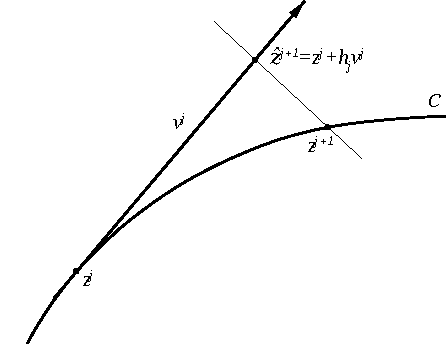
\includegraphics[scale=1.2]{arcstep}
 \caption{\label{fig:pseudo-arc}}
\end{figure}

\section{El mètode de continuació del pseudo-arc}\label{sec:pseudoArc}
Volem trobar punts sobre la corba,
\begin{displaymath}
  \mathcal{C}=\left\{z\in\R^{n+1}: F(z) = 0\right\}
\end{displaymath}
amb $F:\R^{n+1}\longrightarrow \R^{n}$. Suposem conegut 
$z^{j}\in\R^{n+1}$, un punt \emph{regular} de la corba: 
$F(z^{j}) = 0$,  
$\mathop{\mathrm{rang}} DF(z^{j}) = n$. Per a trobar el punt següent,
$z^{j+1}\in\mathcal{C}$, implementarem el mètode del 
pseudo-arc (vegeu~\cite{Kuznetsov2004}, cap.~10, sec.~2) en el dos passos
següents

\begin{enumerate}[label = \emph{\arabic*.}]
  \item \emph{Predicció:} agafarem $\hat{z}^{j+1} = z^{j} + h_{j} v^{j}$ com a
  aproximació del nou punt $z^{j+1}$, on $h_{j}\in\R$ és el pas i
    $v^{j}\in\R^{n+1}$, $\left\|v^{j}\right\| = 1$,
    és el vector tangent a la corba $\mathcal{C}$ al punt $z^{j}$, el qual
    determinarem resolent el \emph{sistema ampliat},  
    \begin{equation}\label{eq:appended_system}
      \begin{split}
      DF\left(z^{j}\right)v &= 0,\\
      \left\langle v^{j-1}, v \right\rangle &= 1, 
    \end{split}
  \end{equation}
    on $v^{j-1}\in\R^{n+1}$, $\left\|v^{j-1}\right\|=1$, és el vector
    tangent a la corba $\mathcal{C}$ al punt $z^{j-1}$, tots dos ($v^{j-1}$
    i $z^{j-1}$) prèviament calculats. Com s'observa
    a~\cite{Kuznetsov2004}:
    \begin{enumerate}[label = (\roman*)] 
      \item El sistema lineal~\eqref{eq:appended_system} és no singular si
	$\mathcal{C}$ és una corba regular (i.e., si
	$\mathop{\mathrm{rang}} DF(z) = n$, $z\in\mathcal{C}$) i els punts
	$z^{j-1}$ i $z^{j}$ estan suficientment a prop.
      \item La solució $v^{\ast}\in\R^{n+1}$ satisfà la condició
	  $\left\langle v^{j-1}, v^{\ast}\right\rangle = 1$, per tant es preserva la
	  direcció al llarg de la corba.
     \end{enumerate}
     Per últim, normalitzem per tenir $v^{j} =
     v^{\ast}/\left\|v^{\ast}\right\|$. \emph{Nota:} a l'inici, quan $j =
     0$, no podrem
     escriure el sistema \eqref{eq:appended_system}, sinó que resoldrem el
     sistema $n\times n$ que s'obté de seleccionar $n$ columnes linealment
     independents
     (siguin les columnes $1,2,\dots,i-1,i+1,\dots,n,n+1$) de
     $DF(z^{j})$ a la primera equació 
     de~\eqref{eq:appended_system} i fixar 
     $v_{i} = 1$. D'aquesta manera trobarem un vector $v^{\ast}\in\R^{n}$, 
     $v^{\ast}_{i} = 1$, t.q.~$DF(z^{0})v^{\ast} = 0$. Llavors $v^{0} =
     \pm v^{\ast}/\left\|v^{\ast}\right\|$, on la tria del signe determinarà
     la direcció en què es continua la corba.

       \item\emph{Correcció}. Per a ``refinar'' el valor aproximat
	 $\hat{z}^{j+1} = z^{j}+h_{j}v^{j}$ del pas predictiu pel mètode de
	 Newton i determinar el nou punt sobre la corba,
	 $z^{j+1}\in\mathcal{C}$, s'ha d'afegir alguna equació addicional
	 al sistema $F(z) = 0$. Al mètode del pesudo-arc, s'imposa que
	 $z^{j+1}\in\hat{z}^{j+1}+ \left\langle
	 v^{j}\right\rangle^{\perp}$; això és, que el punt $z^{j+1}$
	 pertanyi també al hiperplà perpendicular al vector $v^{j}$ que
	 conté $\hat{z}^{j+1}$. Usant el producte escalar aquesta condició
	 geomètrica s'escriu com, 
     \begin{displaymath}
       \left\langle z^{j+1} - \hat{z}^{j+1}, v^{j}\right\rangle =
       \left\langle z^{j+1} - z^{j} - h_{j} v^{j}, v^{j}\right\rangle =
       \left\langle z^{j+1} - z^{j}, v^{j}\right\rangle - h_{j} = 0
     \end{displaymath}
     (vegeu la figura~\ref{fig:pseudo-arc}). Aleshores aplicarem el mètode de
     Newton al sistema no lineal 
     \begin{align*}
       F(z) &=0,\\
       \left\langle z - z^{j}, v^{j}\right\rangle &= h_{j},
     \end{align*}
     prenent $z^{(0)} =\hat{z}^{j+1}$ com a aproximació inicial.
\end{enumerate}

\bibliographystyle{plain}
\bibliography{references}
%\nocite{*}
\end{document}

%%% Local Variables:
%%% mode: latex
%%% TeX-master: "manual"
%%% End:
